\documentclass{beamer}
\usepackage[english]{babel}
\usepackage[utf8]{inputenc}
\usepackage{graphicx}
\usepackage{amsfonts}

\author{Maarten de Jonge}
\title[PGA]{Projective Geometric Algebra}
\subtitle{Supervisor: Leo Dorst}

\newcommand{\rp}{$\mathbb{R}^{3,3}$}

\begin{document}

  \frame{\titlepage}

  \section{Background and Research Question}
  \begin{frame}
    \frametitle{Background}
    \begin{itemize}
      \item GAViewer: Visualisation/calculation tool for GA
      \item Pl\"{u}cker coordinates: Represent lines in $\mathbf{P}^3$ as 6
        coordinates; arises naturally in geometric algebra.
    \end{itemize}

    \begin{center}
      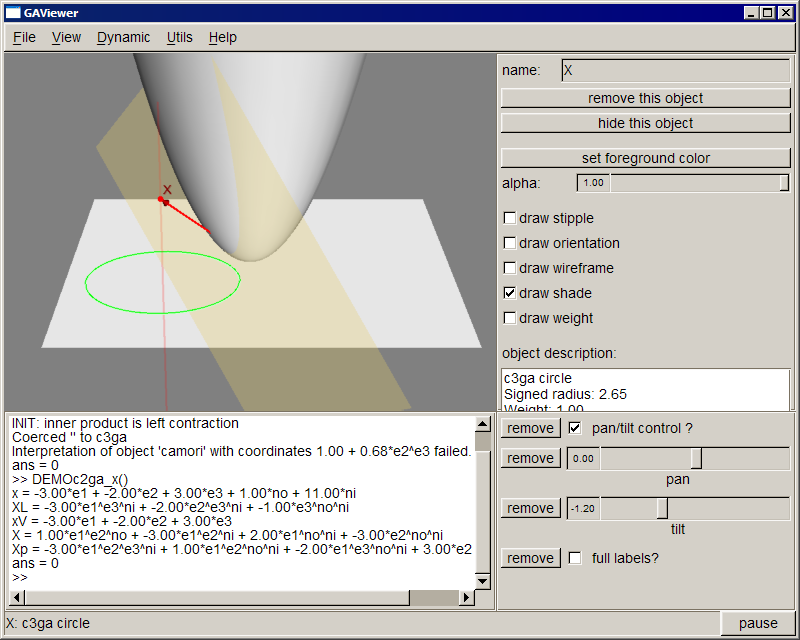
\includegraphics[width=0.7\textwidth]{gaviewer.png}
    \end{center}
  \end{frame}

  \begin{frame}
    \frametitle{Pl\"{u}cker coordinates in \rp}
    \begin{itemize}
      \item Pl\"{u}cker coordinates in GA generalise to \rp\cite{hangbo2011}
      \item vectors in this space represent lines or screw axes in $\mathbf{P}^3$
      \item interpretation and visualisation of the geometrical elements in \rp
      \item Patrick de Kok's bachelor thesis:
        \begin{center}
          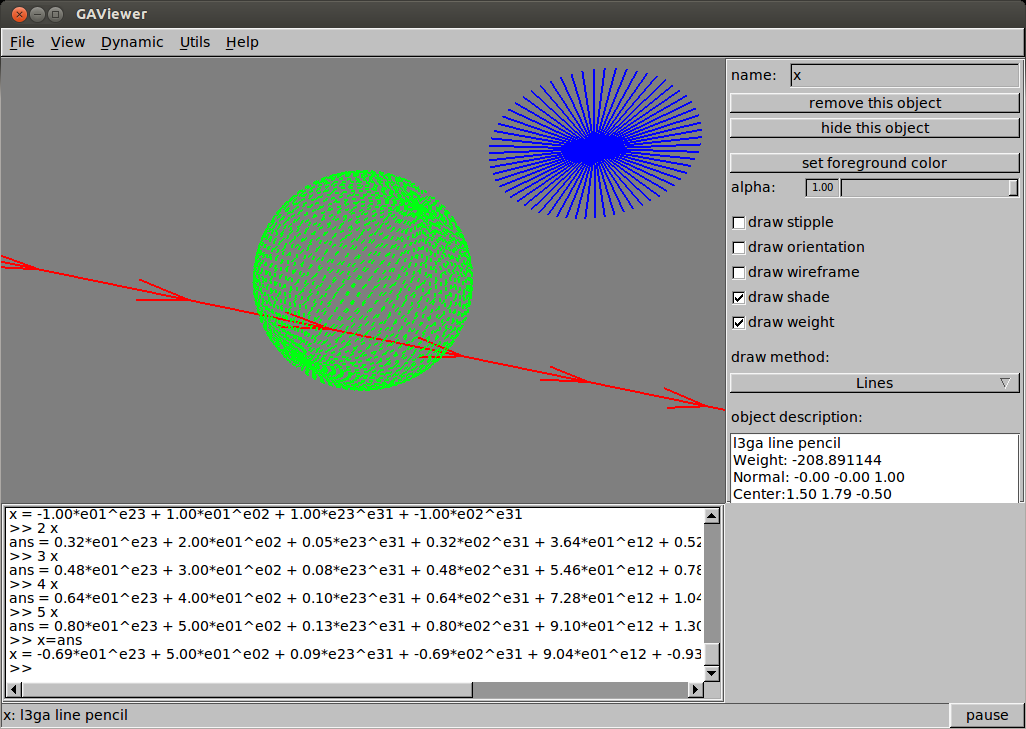
\includegraphics[width=0.7\textwidth]{gaviewer2.png}
        \end{center}
    \end{itemize}
  \end{frame}

  \begin{frame}
    \frametitle{Research Question}
    \begin{itemize}
      \item new developments allow for visualisation of 3-blades of skew lines,
        the \emph{regulus}
        \begin{center}
          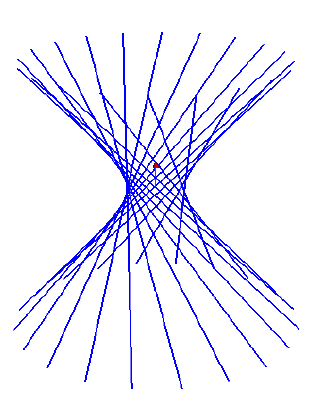
\includegraphics[width=0.3\textwidth]{regulus.png}
        \end{center}
      \item Continue Patrick's work: extend GAViewer with visualisation of the
        regulus
      \item Followed by some application; to be determined soon (a couple of
        options)
    \end{itemize}
  \end{frame}

  \begin{frame}
    \frametitle{Approach}
    The project is easily divisible into a couple of phases:
    \begin{enumerate}
      \item Become familiar with the mathematical background
      \item Implement the visualisation
      \item Follow-up and the corresponding evaluation are yet to be determined
      \item Write report
    \end{enumerate}
  \end{frame}

  \begin{frame}
    \frametitle{Planning}
    \begin{table}
      \begin{tabular}{| l | l |}
        \hline
        week & planning \\
        \hline
        17   & finish maths, decide on follow-up \\
        18   & implement visualisation \\
        19   & finish visualisation if not done yet \\
        20+  & depends on follow-up \\
        \hline
      \end{tabular}
    \end{table}
  \end{frame}

\bibliographystyle{apalike}
\begin{frame}
  \frametitle{References}
  \bibliography{library}
\end{frame}
\end{document}
